\chapter{A data structure for almost-subset queries}
\label{c:trie}

%%%%\documentclass[a4paper,UKenglish,cleveref, autoref, thm-restate]{lipics-v2019}
%%%%%This is a template for producing LIPIcs articles. 
%%%%%See lipics-manual.pdf for further information.
%%%%%for A4 paper format use option "a4paper", for US-letter use option "letterpaper"
%%%%%for british hyphenation rules use option "UKenglish", for american hyphenation rules use option "USenglish"
%%%%%for section-numbered lemmas etc., use "numberwithinsect"
%%%%%for enabling cleveref support, use "cleveref"
%%%%%for enabling autoref support, use "autoref"
%%%%%for anonymousing the authors (e.g. for double-blind review), add "anonymous"
%%%%%for enabling thm-restate support, use "thm-restate"
%%%%
%%%%%\graphicspath{{./graphics/}}%helpful if your graphic files are in another directory
%%%%
%%%%\bibliographystyle{plainurl}% the mandatory bibstyle
%%%%
%%%%\title{A data structure for almost-subset queries}
%%%%
%%%%%\titlerunning{}
%%%%
%%%%\author{James Trimble}{School of Computing Science, University of Glasgow \\ Glasgow, Scotland, UK }{j.trimble.1@research.gla.ac.uk}{https://orcid.org/0000-0001-7282-8745}{}%TODO mandatory, please use full name; only 1 author per \author macro; first two parameters are mandatory, other parameters can be empty. Please provide at least the name of the affiliation and the country. The full address is optional
%%%%
%%%%\authorrunning{J. Trimble} %TODO mandatory. First: Use abbreviated first/middle names. Second (only in severe cases): Use first author plus 'et al.'
%%%%
%%%%\Copyright{James Trimble} %TODO mandatory, please use full first names. LIPIcs license is "CC-BY";  http://creativecommons.org/licenses/by/3.0/
%%%%
%%%%\begin{CCSXML}
%%%%<ccs2012>
%%%%   <concept>
%%%%       <concept_id>10003752.10003809.10003635</concept_id>
%%%%       <concept_desc>Theory of computation~Graph algorithms analysis</concept_desc>
%%%%       <concept_significance>500</concept_significance>
%%%%       </concept>
%%%%   <concept>
%%%%       <concept_id>10003752.10003809.10011254</concept_id>
%%%%       <concept_desc>Theory of computation~Algorithm design techniques</concept_desc>
%%%%       <concept_significance>500</concept_significance>
%%%%       </concept>
%%%% </ccs2012>
%%%%\end{CCSXML}
%%%%
%%%%\ccsdesc[500]{Theory of computation~Graph algorithms analysis}
%%%%\ccsdesc[500]{Theory of computation~Algorithm design techniques}
%%%%
%%%%\keywords{} %TODO mandatory; please add comma-separated list of keywords
%%%%
%%%%%\relatedversion{} %optional, e.g. full version hosted on arXiv, HAL, or other respository/website
%%%%
%%%%\supplement{}
%%%%
%%%%%\funding{(Optional) general funding statement \dots}%optional, to capture a funding statement, which applies to all authors. Please enter author specific funding statements as fifth argument of the \author macro.
%%%%
%%%%%\acknowledgements{}%optional
%%%%
%%%%\nolinenumbers %uncomment to disable line numbering
%%%%
%%%%\hideLIPIcs  %uncomment to remove references to LIPIcs series (logo, DOI, ...), e.g. when preparing a pre-final version to be uploaded to arXiv or another public repository
%%%%
%%%%%Editor-only macros:: begin (do not touch as author)%%%%%%%%%%%%%%%%%%%%%%%%%%%%%%%%%%
%%%%\EventEditors{John Q. Open and Joan R. Access}
%%%%\EventNoEds{2}
%%%%\EventLongTitle{42nd Conference on Very Important Topics (CVIT 2016)}
%%%%\EventShortTitle{CVIT 2016}
%%%%\EventAcronym{CVIT}
%%%%\EventYear{2016}
%%%%\EventDate{December 24--27, 2016}
%%%%\EventLocation{Little Whinging, United Kingdom}
%%%%\EventLogo{}
%%%%\SeriesVolume{42}
%%%%\ArticleNo{23}
%%%%%%%%%%%%%%%%%%%%%%%%%%%%%%%%%%%%%%%%%%%%%%%%%%%%%%%%%%
%%%%
%%%%\usepackage[ruled,vlined]{algorithm2e}
%%%%\usepackage{booktabs}
%%%%\usepackage{tikz}

\newcommand\insertfun{\mathit{insert}}
\newcommand\queryfun{\mathit{query}}
\newcommand\queryHelper{\mathit{queryHelper}}
\newcommand\getOrAddChildNode{\mathit{getOrAddChildNode}}

%%\newcommand{\codelineref}[1]{line~\ref{#1}}
%%\newcommand{\linerangeref}[2]{lines~\ref{#1} to~\ref{#2}}
%%\newcommand{\Lineref}[1]{Line~\ref{#1}}
%%\newcommand{\Linerangeref}[2]{Lines~\ref{#1} to~\ref{#2}}

%%\begin{abstract}
%%This note introduces a data structure, based on a trie, for
%%``almost-subset'' queries.  The data structure stores a collection of sets, and
%%provides a query operation that, given a set $S$ and a number $k$, and returns
%%a list containing each set in the collection that contains at most $k$ elements
%%that are not in $S$.
%%We show how this can be applied a state-of-the-art treewidth solver to
%%give speedups on hard instances.
%%\end{abstract}

\section{Introduction}

Let $\mathcal{C}$ be a collection of subsets of some universe $U$.
A \emph{subset query} on $\mathcal{C}$ takes a query set $Q \subseteq U$ and
returns true if and only if some element of $\mathcal{C}$ is a subset of $Q$.
The enumeration version of the problem returns all subsets of $Q$ that
are in $\mathcal{C}$.  These problems have been well studied
\cite{DBLP:journals/siamcomp/Rivest76,DBLP:conf/ijcai/HoffmannK99,DBLP:conf/icalp/CharikarIP02,DBLP:conf/IEEEares/Savnik13}.
This paper introduces a data structure for a generalised version of the
enumeration problem---the \emph{almost-subset query enumeration problem}---in
which the condition that the the returned sets be subsets of $Q$ is relaxed.
For an integer $k$ provided at query time, any set that
contains no more than $k$ elements that are not in $Q$ is included in the
returned list of sets.

Our data structure closely resembles a Set-Trie
\cite{DBLP:conf/IEEEares/Savnik13}---a data structure for subset and superset
queries.  We add to the Set-Trie a new query operation to allow almost-subset
queries. We also store an additional piece of data in each node of the trie to
enable earlier pruning of subtrees at query time.

As far as I am aware, no data structure for the almost-subset query enumeration
problem has been designed before (although the problem seems so simple that it
would be surprising if it hasn't been looked at before).  However, Tamaki's
state-of-the-art PID algorithm for treewidth \cite{DBLP:journals/jco/Tamaki19}
spends much of its time on an operation that is almost-subset query enumeration
with an additional condition.  For that operation, the PID algorithm uses
a specialised data structure called a \emph{block sieve}.  In this paper, we
show how our new data structure can be straightforwardly augmented to create
a replacement for the block sieve.
Although our data structure uses more memory than the block sieve (I think),
it is much simpler to implement.
Experimental results show that our data structure
outperforms the block sieve on many of the harder treewidth instances from the
2017 PACE Challenge.

\section{Definitions}

For sets $Q$ and $S$, we say that $S$ is a $k$-almost subset of $Q$ if $|S \setminus Q| \leq k$;
that is, $S$ is a subset of $Q$ with at most $k$ additional elements that do not appear in $Q$.
The very closely related concept \emph{almost contains} is introduced by Charikar, Indyk, and Panigrahy
\cite{DBLP:conf/icalp/CharikarIP02} in the context of an algorithm for subset queries.

\section{The data structure}

We assume that the universe $U$, of which the elements of $\mathcal{C}$ are
subsets, is a totally ordered set.  In our examples, we will have $U = \{0, \dots, 7\}$.

The new data structure is a trie, and the layout of the trie is the same as
that of a Set-Trie \cite{DBLP:conf/IEEEares/Savnik13}.  Each set to be stored
in the data structure is viewed as a
string on the alphabet $U$; the characters of the string are the
elements of the set in ascending order.  Thus, for example, the set $\{3,4,5\}$ is
represented as the string 345.  (We will omit quotation marks around strings
for brevity).  Each node of the trie
represents one such string. The root node represents the empty string,
which in turn represents the empty set.  Each string at a non-root node equals the string at
the parent node with one character appended.

Each node carries three pieces of data.  The first of these, $\mathit{char}$,
is the last element of the node's string.  The second is an array (which is of
zero length for leaf nodes) of pointers to child nodes in the trie. The order
of child nodes is unimportant, and simply reflects the order in which sets were
inserted into the data structure.\footnote{Maybe it would be nicer if we kept
them sorted so that the result of a query is sorted?} Finally, each node $N$
contains a Boolean flag $N.\mathit{isElement}$ which is $\mathit{true}$ if
and only if the set represented by node $N$ is contained in the collection.

\Cref{fig:viz1} shows an example of a trie containing the sets
$\{1,3\}$,
$\{3,5,6\}$,
$\{3,5,7\}$,
$\{3,6,7\}$,
$\{1,3,5\}$, and
$\{2,6,7\}$.  The small grey strings will be explained later and can be disregarded
for now.  Nodes that represent sets in the collection, and thus have $\mathit{isElement}=\mathit{true}$,
    are shown with a heavy border.
The bottom-left node in the trie, for example, represents the set $\{3,5,6\}$, which is in the
collection.  The character 6---the last element of the set in ascending order---is
stored at this node.  There is no need to store the full string at each node; we can
reconstruct the set either by following the path from the root to a node and collecting
characters as we go, or by taking advantage of an additional piece of data which we store
at each node, as will be discussed in \Cref{sec:pseudocode}.

\begin{figure}[htb]
\centering
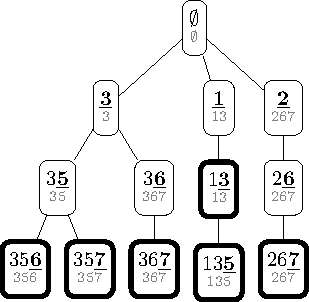
\includegraphics{50-trie/img/viz1}
\caption{A trie containing the sets
$\{1,3\}$,
$\{3,5,6\}$,
$\{3,5,7\}$,
$\{3,6,7\}$,
$\{1,3,5\}$, and
$\{2,6,7\}$.
}
\label{fig:viz1}
\end{figure}

The data structure supports two operations: $\mathit{insert}(S)$ and
$\mathit{query}(Q, k)$.  The algorithm for the $\mathit{insert}()$ operation
begins at the root node and loops over the elements of set $S$ in ascending order,
moving to the corresponding child node for each character, and
creating this node if necessary.  For example, suppose that we wish to insert
the set $\{3,5,7,8\}$ into the trie in \Cref{fig:viz1}.  Beginning at the root
node, we visit child 3, followed by its child 5 (the node labelled 35 in the
figure), followed by its child 7 (the node labelled 357).  Finally, we create a
new child of this node containing the character 8, and set
$\mathit{isElement}=\mathit{true}$ for this node.

The $\mathit{query}(Q, k)$ operation returns all sets in the collection that
contain no more than $k$ elements that are not in $Q$.  Where $k=0$, it is
equivalent to a subset query.
The algorithm that
performs the query operation begins at the root node and performs a depth-first
traversal of the tree.  We have a variable $\mathit{budget}$ which represents
the number of elements not in $Q$ that may be added to the current node's
string.  At the root node, $\mathit{budget}=k$.  When we visit a node whose
character is in $Q$, $\mathit{budget}$ takes the value it had at the parent
node.  When we visit a node whose character is not in $Q$, $\mathit{budget}$ is
one less than its value at the parent node.
If $\mathit{budget}$ is decremented to -1 at a node, this indicates that
the set at this node---and the sets at all descendant nodes---are not $k$-almost
subsets of $Q$, and the algorithm can therefore backtrack.
When backtracking from a child
node to its parent, the value of $\mathit{budget}$ at the parent is restored.

To give an example of the query operation, suppose we wish to find all
1-almost subsets of $\{0,6,7\}$ in the trie in \Cref{fig:viz1}; that is,
all sets stored in the data structure that contain at most one element that 
is not in the set $\{0,6,7\}$.  We call $\mathit{query}(\{0,6,7\}, 1)$ on
the data structure.  The query operation begins at the root node, with a budget
of 1.  It then visits the first child of the root.  Since this child's character
(3) is not in the query set, $\mathit{budget}$ is decremented to zero.
On descending to the the first child of that node (marked 35), budget is
further reduced to -1.  We backtrack to the node marked 3, restore the budget
to 0, and proceed to visit the second child (marked 36).  The algorithm
continues in this way, ultimately returning sets $\{3,6,7\}$ and $\{2,6,7\}$.

\subsection{Subtrie intersections}\label{sec:subtrieintersections}

We use an additional optimisation, which was suggested by Ben Tilly on Stack
Overflow for subset queries \cite{TrieStackOverflow}.  At each search node, we
store a fourth piece of information: the intersection of all the sets with
$\mathit{isElement}=\mathit{true}$ that appear in the subtree rooted at this
node.  This is called $\mathit{intersection}$, and is stored as a bit-string.
In \Cref{fig:viz1}, it is shown as a small grey string.
Thus, for example, we can tell that all sets stored in subtree rooted at the
second child of the root in our example trie contain both 1 and 3.
When $\mathit{query}()$ visits a node, the value $d = |\mathit{intersection} \setminus Q|$ is
calculated.  Since $|S \setminus Q| \geq d$ for
each set stored in the subtree, the algorithm can backtrack if $d > k$.

TODO: give an example of how this can result in exponential speedup.  e.g. all sets
contain the two highest numbers in $U$, and $k=1$.

\subsection{Pseudocode for the operations}\label{sec:pseudocode}

\Cref{InsertAlgorithm} shows pseudocode for the $\insertfun()$ operation.

{
\begin{algorithm}[htb]
 \footnotesize
\DontPrintSemicolon

\nl $\insertfun(S)$ \label{insertfunction} \;
\nl \Begin{
  \nl $\mathit{root}.\mathit{intersection} \gets \mathit{root}.\mathit{intersection} \cap S$ \;
  \nl $\mathit{nodePtr} \gets $ the address of $\mathit{root}$ \;
  \nl \ForEach{$x \in S$ in ascending order} {
      \nl $\mathit{nodePtr} = \getOrAddChildNode(\mathit{nodePtr}, x)$ \;
      \nl $\mathit{nodePtr}.\mathit{intersection} = \mathit{nodePtr}.\mathit{intersection} \cap S$ \;
  }
  \nl $\mathit{nodePtr}.\mathit{isElement} \gets \mathit{true}$ \;
}

\nl $\getOrAddChildNode(\mathit{nodePtr}, x)$ \;
\nl \Begin{
  \nl \ForEach{$\mathit{childPtr} \in \mathit{nodePtr}.\mathit{children}$} {
      \nl \If {$\mathit{childPtr}.\mathit{char} = x$} {
          \nl \KwSty{return} $\mathit{childPtr}$ \;
      }
  }
  \nl Create a new child of the node pointed to by $\mathit{nodePtr}$, with $\mathit{char} = x$ and $\mathit{intersection} = U$ \;
  \nl \KwSty{return} this new child \;
}
\caption{The $\insertfun()$ operation}
\label{InsertAlgorithm}
\end{algorithm}
}

\Cref{QueryAlgorithm} shows pseudocode for the $\queryfun()$ operation and a
recursive helper function, $\queryHelper()$, that traverses the trie in depth
first order.  The function $\queryHelper()$ takes a pointer to a trie node, the
query set $Q$, and the remaining budget, and returns the variable
$\mathit{sets}$, which is a list of all the sets in the subtree rooted at the
given trie node that satisfy the query.

\Lineref{subtrieOptimisationLine} uses the subtrie-intersection optimisation
described in \Cref{sec:subtrieintersections} to backtrack early.  The algorithm
would remain correct even if this line were removed, but would possibly visit
more nodes of the trie.

\Lineref{outputSet} adds a node's set to the output collection of sets if
$\mathit{isElement}$ is $\mathit{true}$.  This line takes advantage of the
fact that if a node's set $S$ is an element of the collection
then the node's $\mathit{intersection}$ equals $S$ (since a node's set
is a subset of every set that appears in the subtree rooted at that node).

The loop beginning on \codelineref{queryChildLoop} tries each child node in turn,
and visits those nodes that do not break the budget constraint.

{
\begin{algorithm}[htb]
 \footnotesize
\DontPrintSemicolon
\nl $\queryfun(Q,k)$ \label{queryfunction} \;
\nl \Begin{
    \nl $\mathit{rootPtr} \gets$ the address of $\mathit{root}$ \;
    \nl \KwSty{return} $\queryHelper(\mathit{rootPtr}, Q, k)$
}

\nl $\queryHelper(\mathit{nodePtr}, Q,\mathit{budget})$ \label{queryhelperfunction} \;
\nl \Begin{
  \nl \lIf{$|\mathit{nodePtr}.\mathit{intersection} \setminus Q| > k$} {\KwSty{return} $\emptyset$ \label{subtrieOptimisationLine}}
  \nl $\mathit{sets} \gets \emptyset$ \;
  \nl \lIf{$\mathit{nodePtr}.\mathit{isElement}$} {$\mathit{sets} \gets \{\mathit{nodePtr}.\mathit{intersection}\}$ \label{outputSet}}
  \nl \ForEach{$\mathit{childPtr} \in \mathit{nodePtr}.\mathit{children}$ \label{queryChildLoop}} {
      \nl \lIf {$\mathit{childPtr}.\mathit{char} \in Q$}{$\mathit{newBudget} \gets \mathit{budget}$}
      \nl \lElse {$\mathit{newBudget} \gets \mathit{budget} - 1$}
      \nl \If {$\mathit{newBudget} \geq 0$} {
        \nl $\mathit{sets} \gets \mathit{sets} \cup \queryHelper(\mathit{childPtr}, Q, \mathit{newBudget})$
      }
  }
  \nl \KwSty{return} $\mathit{sets}$
}
\caption{The $\queryfun()$ operation}
\label{QueryAlgorithm}
\end{algorithm}
}

TODO: say how my implementation differs slightly in how $\mathit{intersection}$
is created for new nodes.  Say how else my implementation differs.

\subsection{A small experiment}

This section presents a very small-scale experiment to test the effectiveness
of the new data structure.
The implementations were in Java, and I ran the experiment on my laptop.
For each $k \in \{0, \dots, 10\}$, I randomly generated
100,000 10-element subsets of $U = \{0, \dots, 49\}$ and added them to a trie
data structure.  I then performed 1000 $(S, k)$ queries, with each set $S$
being a randomly generated set of size 10.  I ran the same set of additions
and queries using Java's HashSet data structure; the queries were performed
by iterating over all elements $S$ of the HashSet and testing whether the union
of the query set and $S$ had cardinality at most $10 + k$.

\Cref{table:experiment1} shows the results.  The \emph{Items} column shows the
mean number of items returned per query, and the final two columns show total
run times in milliseconds for the HashSet and trie.  In each case, the total
time to add all elements to a collection (which is not shown in the table) was
less than 150 ms; thus, in almost all cases the query time made up by far the
greater part of the total run time.  For $k \leq 3$, the trie required less
time than the HashSet.  For larger values of $k$, the HashSet was faster.  In
these cases, many sets were output, and the slow run times using the trie can
be explained by the overhead of traversing the tree and reconstructing sets
from the characters at nodes.

\begin{table}[h]
    \centering
    \begin{tabular}{lrrrrr}
\toprule
$k$ & Items & \multicolumn{2}{c}{Time (ms)} \\
\cmidrule(r){3-4}
 & & Hash set & Trie \\
\midrule
0 & 0.001 & 6122 & 135 \\
1 & 0.051 & 5860 & 363 \\
2 & 2.344 & 5874 & 1697 \\
3 & 59.670 & 6273 & 4331 \\
4 & 741.144 & 5895 & 7969 \\
5 & 4973.981 & 5992 & 12293 \\
6 & 19682.141 & 6220 & 16800 \\
7 & 48501.369 & 6852 & 24440 \\
8 & 79580.199 & 6703 & 29796 \\
9 & 96445.432 & 6768 & 32230 \\
10 & 99990.000 & 6448 & 32046 \\
\bottomrule
\end{tabular}

    \caption{Comparison of hash set and trie for almost-subset queries.
        For each value of $k$ from 0 to 10, we added 100,000 sets of size 10
        to a collection, then performed 1000 queries.  Each query sought,
        for a randomly generated set of size 10, 
        all $k$-almost subsets of $S$ in the collection.  The \emph{Items}
        column shows the mean number of items returned from the collection
        per query.  The final two columns show the total time (for
        100,000 additions and 1000 queries) for the hash set and trie data
        structures.}
    \label{table:experiment1}
\end{table}

\section{Application to treewidth}

In this section, we use our trie as a replacement for a data structure within
Tamaki's PID program, which is a state-of-the-art algorithm for the exact
treewidth problem \cite{DBLP:journals/jco/Tamaki19}.  The solver came second in
the exact track of the PACE Challenge 2017 \cite{DBLP:conf/iwpec/DellKTW17},
and had the fastest overall run time.  The same author presents a family of
three algorithms in another recent paper \cite{DBLP:conf/sea2/Tamaki19}.
While these perform extremely well on certain classes of graph, my small-scale
experiments (and for a few instances, the results in the paper) show that they
do not dominate the PID algorithm on all graphs.  Thus, the PID solver
is a good example of a leading solver in which we can test the performance
of our data structure.

\subsection{Data structure interface required by PID}

The data structure used by PID to store sets, which is called a \emph{block
sieve}, is constructed for a particular graph $G$ and an integer $k$, and stores subsets
of the vertex set of $G$.  The data structure has two operations.  The first,
$\mathit{store}(S)$, adds set $S$ to the block sieve if it is not already present.
The second, $\mathit{supersets}(Q)$, returns a list containing $N(S)$ for each set
$S$ in the block sieve such that $Q \subseteq S$ and $|N(Q) \cup N(S)| \leq k + 1$,
where the neighbourhood operator $N(S)$ gives the set of vertices that are adjacent
in $G$ to some vertex in $S$ but are not themselves in $S$.

The second of these conditions---that $N(S)$ contains few elements that do not
appear in $N(Q)$---is the same as the almost-subset condition.  This suggests
that we could modify our almost-subset trie data structure to carry out the
role of the block sieve.  We now turn to this task.

\subsection{Modifications to our trie}

To use our trie in the PID algorithm, we store the neighbourhood $N(S)$ in the
data structure when $\mathit{store}(S)$ is called.  We also need to store the set
$S$ at the node whose key is $N(S)$.  Therefore, we replace the Boolean flag
$\mathit{isElement}$ in each node of the trie with a (possibly empty) array $\mathcal{S}$
of sets.  When adding $S$ to the data structure, we add $S$ to the $\mathcal{S}$
array of the node corresponding to $N(S)$.

The modification to the $\mathit{query}$ operation is then very
straightforward: at \codelineref{outputSet} of \Cref{QueryAlgorithm}, we simply
need to loop over the sets in $\mathcal{S}$, and make the assigment
$\mathit{sets} \gets \{\mathit{nodePtr}.\mathit{intersection}\}$ if any of
these sets is a superset of the query set.

We add one further optimisation.  In addition to storing at each node the
intersection of neighbourhoods ($N(S)$ sets) that appear in the subtrie rooted
at that node, we also store the union of $S$ sets that appear in the subtrie.
After \codelineref{subtrieOptimisationLine}, we are then able to check whether
this union is a superset of the query set, and return an empty set if it is
not.

\Cref{fig:viz2} shows the trie data structure after these modifications.
The trie shown is the final trie data structure created while running the PID
algorithm on the Petersen graph, with vertices labelled from 0 to 9.
The bottom-left node, for example, represents the set $\{3,4,6\}$ and its
neighbourhood $\{0,2,5,7,8,9\}$.

\begin{figure}[htb]
\centering
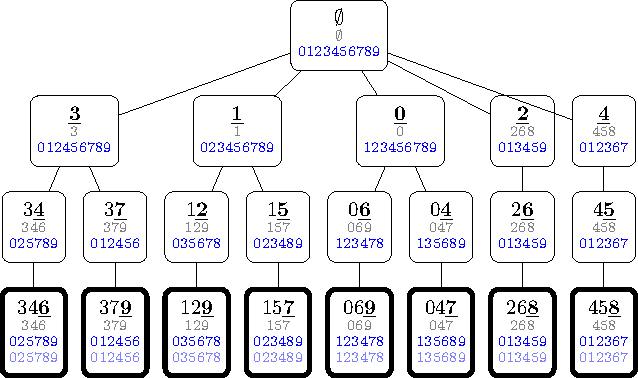
\includegraphics{50-trie/img/Petersen}
\caption{The trie data structure after modifications for the PID application.
Light blue strings represent $S$ sets stored at the node.  Each dark blue string
is the union of $S$ sets in the subtree rooted at that node.}
\label{fig:viz2}
\end{figure}

Although the block sieve does use tries, there are numerous differences between
our approach and the block sieve:

\begin{itemize}
  \item It is necessary to use a list of block sieves, whereas our data structure
    requires a single trie.
  \item In the block sieve, the keys are sets $S$, whereas we use their neighbourhoods
    $N(S)$ as keys.
  \item Our trie branches on single vertices, whereas the block sieve branches
    on subsets of vertices (actually, substrings of a bitset).
  \item The parameter $k$ is fixed at the construction of the block sieve, whereas
    with the new trie it can be set to a different value on each query.
\end{itemize}

TODO time and space trade-offs.  My data structure is memory-hungry :-(

\subsection{Implementation details}

TODO: bitsets etc.

\subsection{Experiment}

Tamaki's implementation of the PID algorithm is in
Java.\footnote{\url{https://github.com/TCS-Meiji/PACE2017-TrackA}}  I have
implemented the new trie data structure in Java and used it as a replacement
for the block sieve in Tamaki's PID
    program.\footnote{\url{https://github.com/jamestrimble/PACE2017-TrackA/blob/master/tw/exact/NewTrie.java}}
    It is only 100 lines of code (if you delete the code for creating LaTeX
    visualisations of the tries).
    I ran the original PID program and my modified version with a 5 GB memory
    laptop on my four-year-old laptop.  \Cref{fig:scatter} shows the run times
    for the 100 highest-numbered PACE 2017 instances.  The new data structure
        seems to improve run times for most of the harder instances.  There is
        one exception where my program runs out of memory.

TODO experiments on random instances

\begin{figure}[htb]
\centering
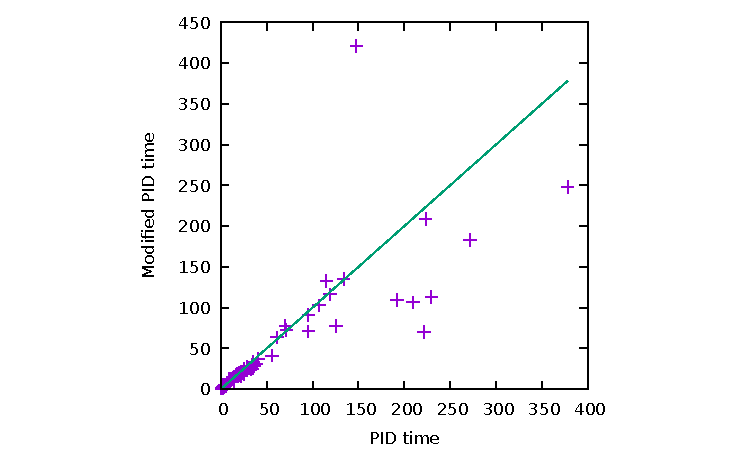
\includegraphics{50-trie/img/plot}
\caption{Run times on 100 PACE Challenge instances.  On the horizontal axis,
run time for Tamaki's PID program.  On the verical axis, run time for Tamaki's
PID program with an augmented version of the new trie data structure used
instead of a block sieve.}
\label{fig:scatter}
\end{figure}

\section{Compressing the trie}

I haven't written this section yet, but I've written the code.  It seems to save
memory but doesn't save much time.  The idea of the compressed trie is in
\Cref{fig:vizc2}.

\begin{figure}[htb]
\centering
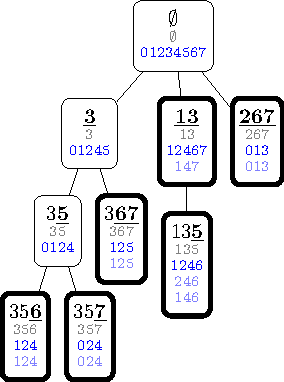
\includegraphics{50-trie/img/vizc2}
\caption{A compressed trie}
\label{fig:vizc2}
\end{figure}

%%%\section{Notes to self}
%%%
%%%\cite{DBLP:conf/IEEEares/Savnik13}
%%%\cite{DBLP:conf/ijcai/HoffmannK99}
%%%
%%%\cite{DBLP:journals/siamcomp/Rivest76}
%%%\cite{DBLP:conf/icalp/CharikarIP02} defines almost contains!!!


%%\bibliography{bib}
